\documentclass{article}
\usepackage[utf8]{inputenc}
\usepackage[greek,english]{babel}
\usepackage{alphabeta}
\usepackage{fancyhdr}
\usepackage{listings}
\usepackage{mathtools}
\usepackage{xcolor}
\usepackage{graphicx}
\usepackage{siunitx}
\usepackage{float}

\title{Ενσωματωμένα Συστήματα - Τελική Εργασία}
\author{Χρήστος Μαργιώλης - 19390133}
\date{Ιανουάριος 2022}

\begin{document}

\begin{titlepage}
        \maketitle
        \begin{figure}[t!]
        \begin{center}
        
\includegraphics[scale=0.3]{./res/uniwalogo.png} \\
        \Large
        \textbf{Πανεπιστήμιο Δυτικής Αττικής} \\
        \large
        Τμήμα Μηχανικών Πληροφορικής και Ηλεκτρονικών Υπολογιστών
        \end{center}
        \end{figure}
\end{titlepage}

\renewcommand{\contentsname}{Περιεχόμενα}
\tableofcontents
\pagebreak

\section{Πληροφορίες}
\subsection{Λίστα υλικών -- BOM}
\begin{itemize}
	\item Microchip PIC16F877A - I/P μικροελεγκτής.
	\item Adafruit BME280 σένσορας θερμοκρασίας, υγρασίας και πίεσης.
	\item 16x2 LCD οθόνη.
	\item 1x \SI{16}{\mega\hertz} κρυσταλλικός ταλαντωτής.
	\item 2x \SI{10}{\kohm} αντίσταση.
	\item 2x \SI{330}{\ohm} αντίσταση.
	\item 1x \SI{10}{\kohm} ποτενσιόμετρο.
	\item 2x \SI{22}{\pico\farad} κεραμεικός πυκωντής.
	\item 2x LED
	\item 2x κουμπί.
	\item Καλώδια.
	\item 3x AAA μπαταρίες (4.5V) ή μπαταρία 9V με 5V διαιρέτη τάσης.
\end{itemize}

\subsection{Κόστος παραγωγής}

Οι τιμές υπολογίστηκαν με βάση τα τιμολόγια του https://www.digikey.com. \\

Για 100 τεμάχια:
\begin{center}
\begin{tabular}{|l|l|}
	\hline
	\textbf{Μέρος} & \textbf{Τιμή} \\ 	
	\hline
	PIC16F877A	& \$706 \\
	BME280		& \$1495 \\
	LCD		& \$365 \\
	\hline
	Σύνολο		& \$2566 \\
	\hline
\end{tabular}
\end{center}

Για 1500 τεμάχια:
\begin{center}
\begin{tabular}{|l|l|}
	\hline
	\textbf{Μέρος} & \textbf{Τιμή} \\ 	
	\hline
	PIC16F877A	& \$10.590 \\
	BME280		& \$22.420 \\
	LCD		& \$5.470 \\
	\hline
	Σύνολο		& \$38.480 \\
	\hline
\end{tabular}
\end{center}

'Οχι και ό,τι πιο οικονομικό έχει βγει...

\subsection{Θερμοκρασίες λειτουργίας}

\begin{center}
\begin{tabular}{|l|l|}
	\hline
	\textbf{Μέρος} & \textbf{Εύρος θερμοκρασίας} \\ 	
	\hline
	PIC16F877A	& $\SI{-40}{\celsius} \sim \SI{85}{\celsius}$ \\
	BME280		& $\SI{-40}{\celsius} \sim \SI{85}{\celsius}$ \\
	LCD		& $\SI{-20}{\celsius} \sim \SI{70}{\celsius}$ \\
	\hline
\end{tabular}
\end{center}

Οπότε, παίρνοντας υπόψη την οθόνη LCD η οποία έχει το μικρότερο
εύρος θερμοκρασίας λειτουργίας, το σύστημα είναι ασφαλές να
λειτουργήσει στους $\SI{-20}{\celsius} \sim \SI{70}{\celsius}$.

\subsection{Διάρκεια ζωής}

<++>

\section{Ανάπτυξη συστήματος}
\subsection{Εργαλεία}
Η ανάπτυξη του συστήματος έγινε σε FreeBSD 13.0 με την χρήση του
\lstinline{sdcc} C compiler, και το \lstinline{pk2cmd} για την
επικοινωνία του μικροελεγκτή με το PICKit2 -- τον προγραμματιστή.
'Εχω αναλύσει την διαδικασία αυτή σε μορφή οδηγού στην ιστοσελίδα
μου και στο FreeBSD Wiki: https://wiki.freebsd.org/Microcontrollers/PIC

\subsection{Σχηματικό}
\begin{center}
	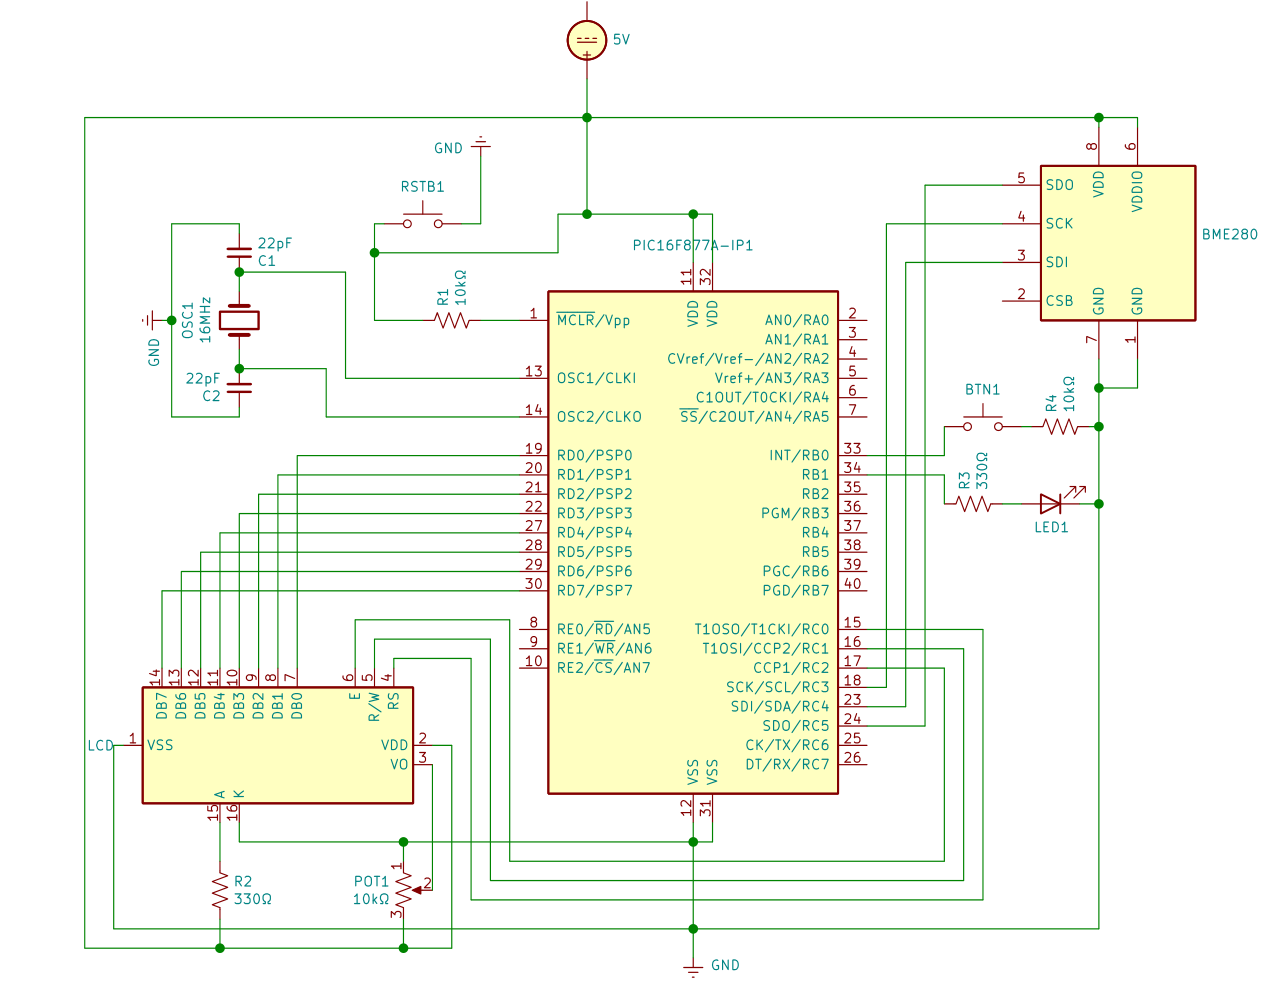
\includegraphics[width=\linewidth]{./res/schem.png}
\end{center}

\subsection{PCB}
<++>

\subsection{Κώδικας}
<++>

\subsection{Εικόνες}
<++>

\end{document}
